\documentclass[lettersize,journal]{IEEEtran}
\usepackage{amsmath,amsfonts}
\usepackage{algorithmic}
\usepackage{algorithm}
\usepackage{array}
\usepackage[caption=false,font=normalsize,labelfont=sf,textfont=sf]{subfig}
\usepackage{textcomp}
\usepackage{stfloats}
\usepackage{url}
\usepackage{verbatim}
\usepackage{graphicx}
\usepackage{cite}

\hyphenation{op-tical net-works semi-conduc-tor IEEE-Xplore}

\begin{document}
\title{Generating adversarial examples using Generative Adversarial Network (GAN)}

\author{Yeganeh Morshedzadeh}

\maketitle

\begin{abstract}
Since much research has been made on the vulnerability of Deep neural networks (DNNs), we tried to generate more realistic and efficient adversarial examples in this project.	More precisely, we used the Adv-GAN framework to learn and approximate the distribution of original instances. Afterward, we used the generator to produce high perceptual quality adversarial examples once the Adv-GAN was trained. The generator can be efficiently and independently used to generate adversarial perturbations for any given instance. Therefore, this attack can be used in both semi-white-box and black-box attacks. Using this method we could perform a 99.57\% attack success rate on the target model, which had a 99.3\% accuracy on the MNIST dataset before the attack. 
\end{abstract}

\begin{IEEEkeywords}
Generative Adversarial Network, Adversarial Example, Fast Gradient Sign Method, Adversarial Perturbations, Deep neural networks.
\end{IEEEkeywords}

\section{Introduction}
\IEEEPARstart{C}urrently, deep learning (DL) along with other machine learning (ML) and artificial intelligence (AI) methods have made remarkable advancements in providing solutions to challenging scientific problems at a large scale, such as reconstructing brain circuits \cite{Helmstaedter2013ConnectomicRO} and analyzing mutations in DNA \cite{Xiong2015TheHS}. In addition, deep neural networks (DNNs) have become the preferred choice of researchers when tackling many challenging problems in speech and voice recognition \cite{Hinton2012DeepNN}, natural language understanding \cite{Sutskever2014SequenceTS}, and computer vision.

Continuous advancements in deep neural network models \cite{Szegedy2016RethinkingTI, He2016DeepRL}, open access to DL software libraries \cite{Vedaldi2015MatConvNetCN, Jia2014CaffeCA, Abadi2016TensorFlowLM}, and easy access to the required hardware for training complex models have helped DL quickly reach a level of maturity for entry into sensitive and critical applications such as self-driving cars, surveillance systems \cite{Najafabadi2014DeepLA}, malware detection \cite{Papernot2016TowardsTS, Grosse2017AdversarialEF}, robots and drones \cite{Mnih2015HumanlevelCT, Giusti2016AML}, voice command recognition \cite{Hinton2012DeepNN}, and face ID security on mobile devices.

In some cases, these applications are so important that an individual's life and property depend on them \cite{Madry2018TowardsDL}. For example, an attacker could mislead an autonomous vehicle or compromise the intelligent agents that communicate via voice commands. Research has shown that machine learning algorithms are vulnerable to adversarial examples. These examples, obtained by slight and imperceptible perturbations in the dataset samples, can mislead the classifier model \cite{Akhtar2018ThreatOA}. 

Considering that in most research, the goal has been to increase the accuracy of the network and less attention has been paid to the security and flexibility of the model, even for the most powerful trained networks with very high accuracy in image classification, one can find adversarial examples that mislead the network into predicting with confidence and misleading it. Therefore, ensuring the robustness and security of deep learning models is of great importance.

\subsection*{An example of the importance of adversarial examples.}
Imagine a self-driving car approaching an intersection and approaching a stop sign but instead of reducing speed, it increases its speed and as a result, an accident occurs. Later, a reporter reveals that there were four rectangles glued onto the stop sign, which caused the AI of the car to mistakenly recognize it as a speed limit of 45. This real example was presented by scientists who were able to mislead the AI system by placing labels on the stop sign \cite{Evtimov2017RobustPA}. 
In the image on the left of fig. \ref{stop_speed}, by placing labels, the image is transformed into the image on the right, which, although easily recognizable by humans, is recognized by AI systems as a 45 speed limit sign instead of a stop sign, which is very dangerous \cite{Heaven2019DLFool}.

\begin{figure}[!t]
\centering
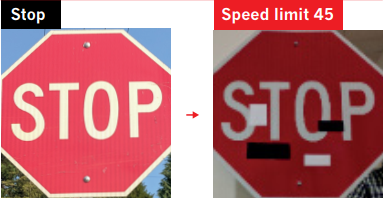
\includegraphics[width=2.5in]{stop_speed.PNG}
\caption{An example of error in neural networks in detecting traffic signs \cite{Evtimov2017RobustPA}.}
\label{stop_speed}
\end{figure}


\section{Background}
\subsection*{Adversarial Example  \& Adversarial Training}
An adversarial example/image is a modified version of a sample, for example, an image that is intentionally and knowingly distorted and manipulated to mislead the network.

These examples are created by adversarial perturbations, which are small changes in the original image that are imperceptible or quasi-imperceptible to humans but appear entirely different to networks.

Adversarial training is the use of adversarial examples alongside clean and untouched samples to train deep learning models.

\subsection*{Classification of Adversarial Attacks}
Adversarial attacks are classified into different categories, such as targeted attacks and untargeted attacks, universal attacks and data-dependent attacks, perturbation attacks and replacement attacks, black-box attacks, semi-white-box attacks, and white-box attacks.

\subsubsection*{White-Box Attacks}
In this type of attack, it is assumed that complete knowledge about the target model, parameter values, architecture, training method, and in some cases, training data, is available.

\subsubsection*{Black-Box Attacks}
In black-box attacks, adversarial examples that are created without any knowledge of the target model are presented to the target model during the testing phase. In some cases, it is assumed that the attacker has limited knowledge about the model, such as the training process or architecture, but certainly knows nothing about the model's parameters.

\subsubsection*{Semi-White-Box Attacks}
In this type of attack, which is very similar to black-box and white-box attacks, any other knowledge or information about the target model is used. For example, probabilities obtained from the network's predictions can be used as additional information whereas in black-box attacks could be using only the final prediction, i.e. predicted class.

\subsection*{Generative Adversarial Network}
Generative Adversarial Network (GAN) \cite{Goodfellow2014GenerativeAN}, consists of two main parts called generator and discriminator. These two neural networks have opposite functions and compete with each other in a zero-sum game.
Originally, this network was introduced as a generative model for unsupervised learning, but generative adversarial networks have proven to be useful for semi-supervised learning, supervised learning, and reinforcement learning.
\subsubsection*{Generator}
The generator takes a noise, often in the form of Gaussian or uniform, as its input and then produces a very noisy image of the input data. The main goal of the generator is to produce images that are as similar as possible to natural and realistic images in the dataset.

The generator produces images with the same dimensions as the images in the dataset from random noise.

\subsubsection*{Discriminator}
The discriminator takes an image as its input and its task is to distinguish between real images, images in the dataset, and fake images, generated by the generator.

If the discriminator recognizes the image as natural, it gives a value close to 0 in the output, and if it recognizes the image as unnatural, it gives a value close to 1 in the output.

\subsubsection*{How does a GAN work?}
The main goal of the Generative Adversarial Network is to generate an image that is as natural as possible to the extent that it can deceive both computers and humans. As shown in fig. \ref{ganArch}, the images generated by the generator and the images in the dataset are fed to the discriminator. The discriminator's goal is to distinguish between the two types of images, while the generator's goal is to produce images that can deceive the discriminator. Specifically, the generator first produces some natural and convincing images, and then after calculating the gradients, these values are used to update the parameters of both networks.

\begin{figure}[!t]
\centering
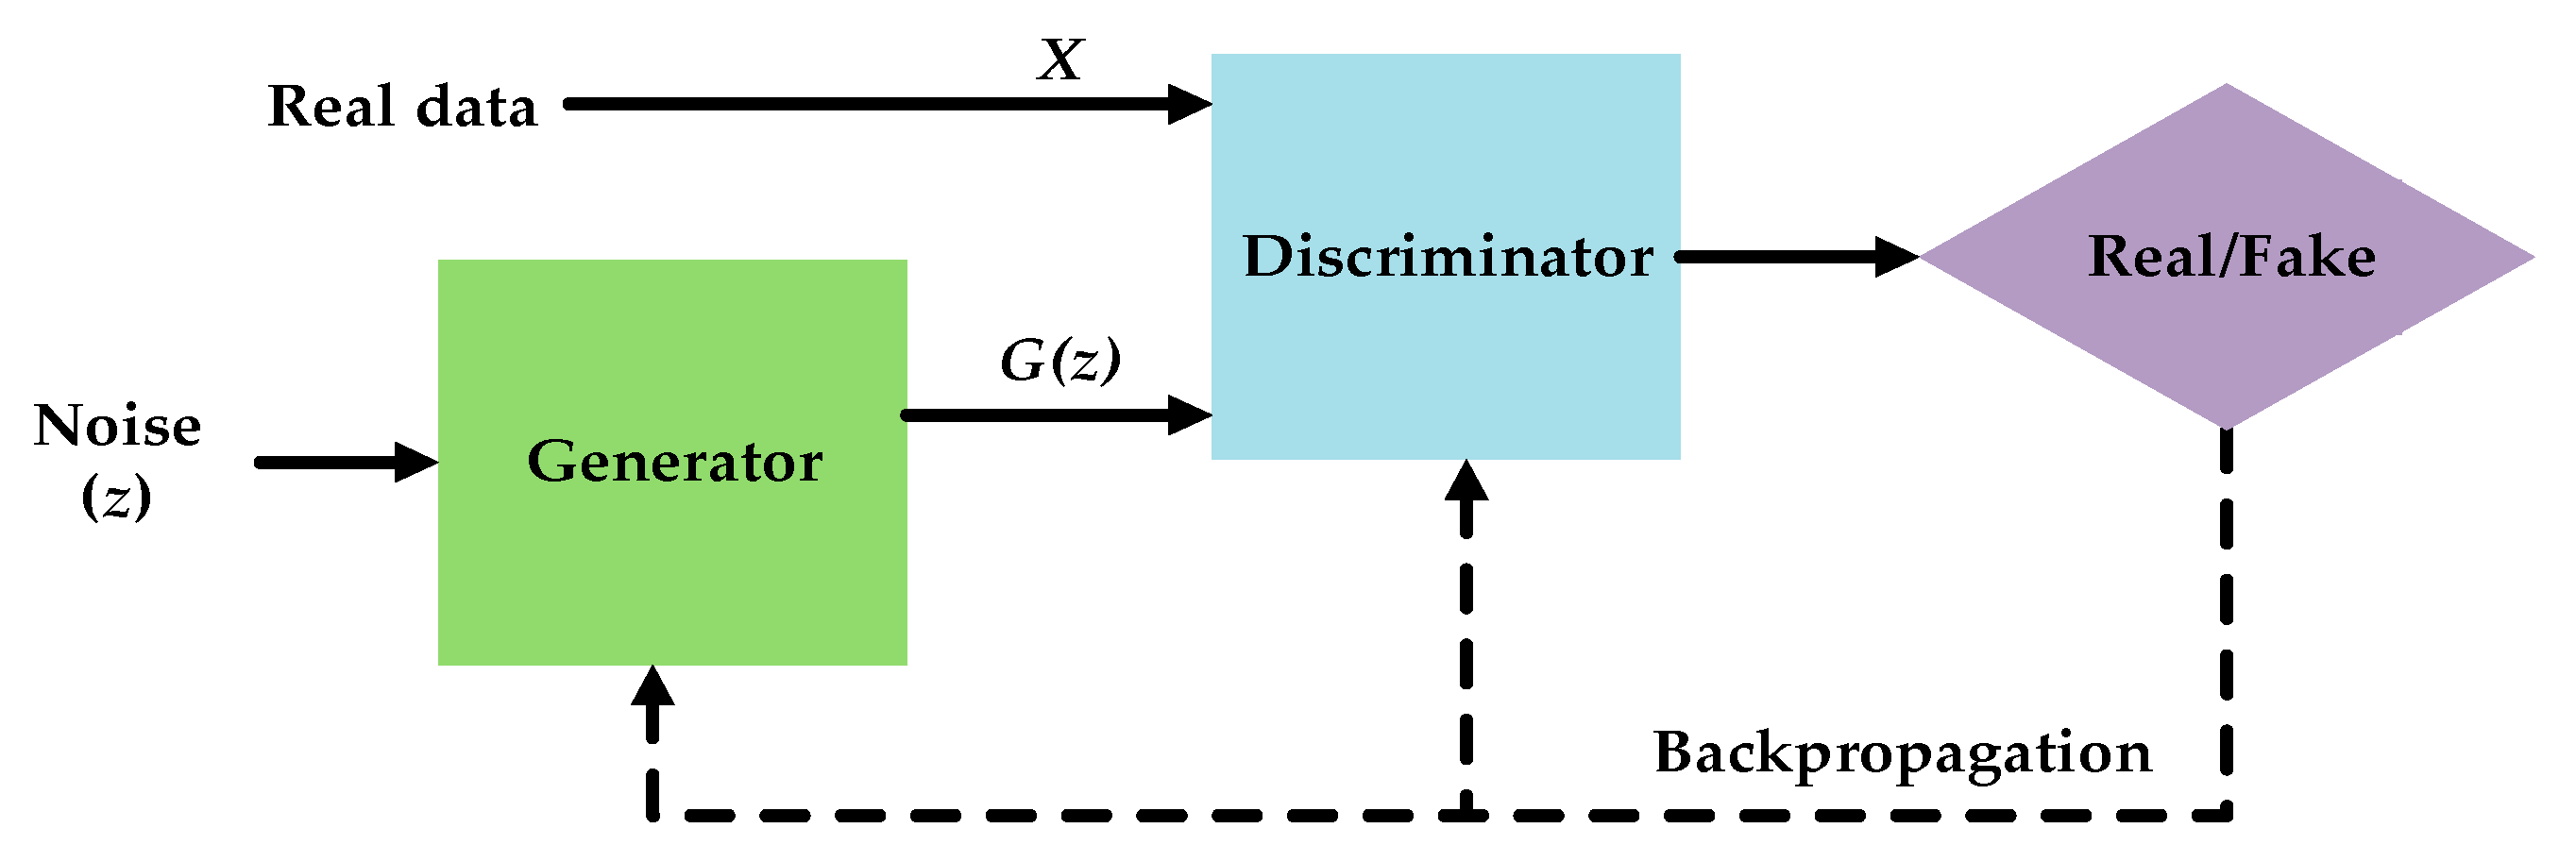
\includegraphics[width=3.5in]{ganArch.PNG}
\caption{Architecture of a GAN \cite{Goodfellow2014GenerativeAN}}
\label{ganArch}
\end{figure}

In fig \ref{ganlab}, a visualization of the interaction and training process of a generative adversarial network is shown\footnote{This can be accessed through {https://poloclub.github.io/ganlab/}}.

\begin{figure}[!t]
\centering
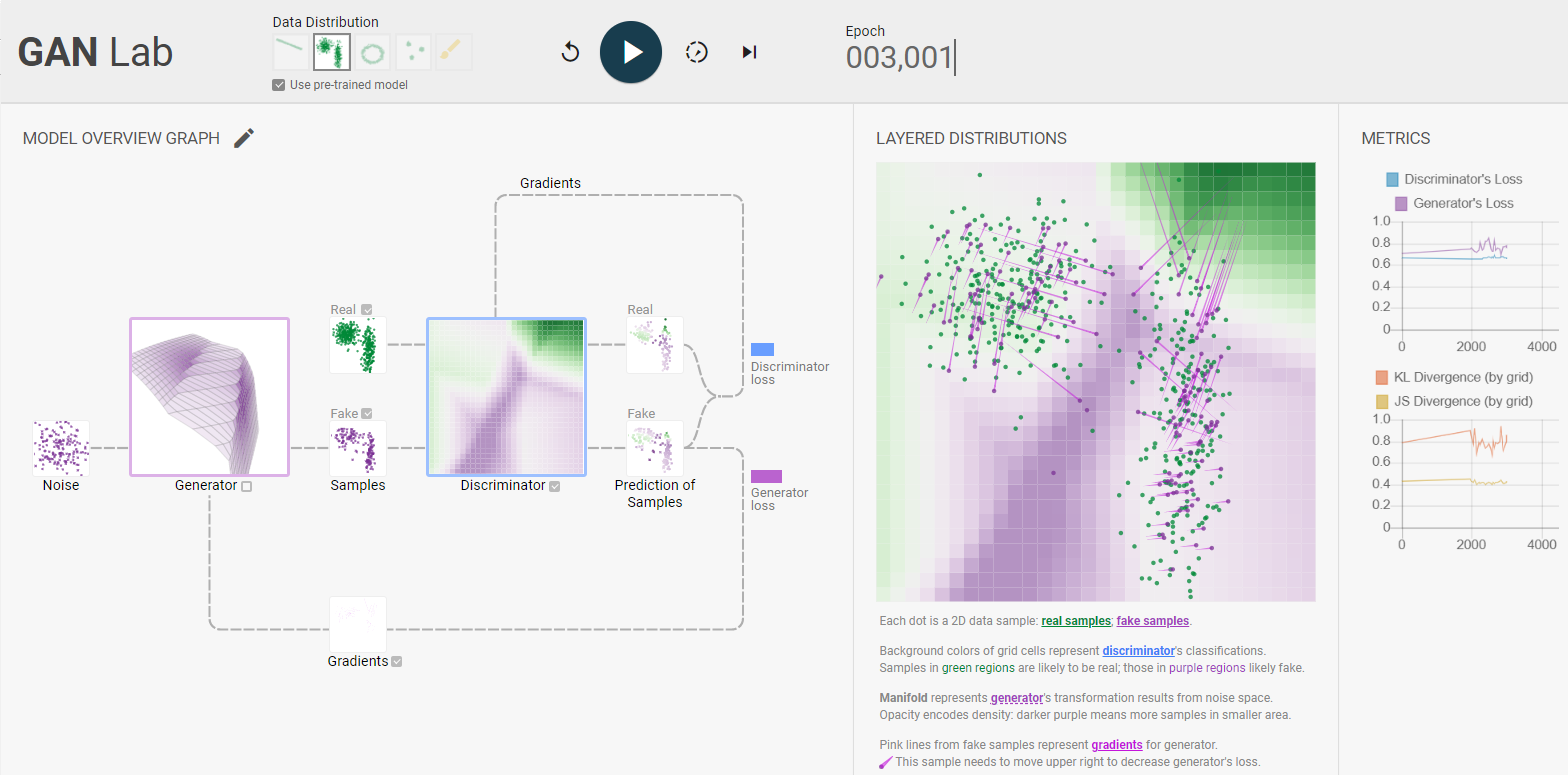
\includegraphics[width=3.5in]{ganlab.PNG}
\caption{Visualization of how a GAN works.}
\label{ganlab}
\end{figure}

\section{Review of Related Work}
To attack neural networks, DNNs can be exposed to adversarial examples.  By adversarial training, the robustness and strength of the network can be increased. The following methods have been proposed for attacks:

\begin{list}{-}{}
\item Fast Gradient Sign Method (FGSM) \cite{Goodfellow2015ExplainingAH}, \cite{Kurakin2017AdversarialEI}: 
\item Projected Gradient Descent (PGD) \cite{Kurakin2017AdversarialML}
\item Carlini and Wagner Attack (C\&W) \cite{Carlini2017TowardsET}
\item One-pixel attack \cite{Su2019OnePA}
\item Basic Iterative Method (BIM) \cite{Kurakin2017AdversarialEI}
\item DeepFool \cite{MoosaviDezfooli2016DeepFoolAS}
\end{list}


\subsection*{Fast Gradient Sign Method Algorithm}

One of the effective methods proposed for adversarial training is the FGSM \cite{Goodfellow2015ExplainingAH}, which optimally calculates an adversarial manipulation for an image.

This method is part of the white-box attacks because the adversary needs access to the architecture and parameters of the model at all times.

\subsubsection*{Equation}

The equation for the FGSM algorithm is as follows:

\begin{equation} \label{eq:fgsm}
X^{adv} = X + \epsilon \cdot sign(\nabla_XJ(X, Y_{true}))
\end{equation}

In equation (\ref{eq:fgsm}), we have:
\begin{itemize}
\item $X$: the original and unchanged image
\item $X^{adv}$: the adversarial example that is obtained after applying the FGSM to the original image
\item $\epsilon$: a constant to determine the severity of the attack (the size of the adversarial perturbation)
\item $J$: the loss function
\item $Y_{true}$: the actual class and label of the original image
\item $\nabla_X$: the gradient of the cost function
\end{itemize}
In this equation (\ref{eq:fgsm}), the larger the value of $\epsilon$, the more the adversarial example deviates from the original image.

\subsubsection*{How the algorithm works?}

The goal of this method is to add a calculated noise, which is not random and is in the direction of the cost function's slope in the original image. In this method, the attacker exactly benefits from the method used to train the network in detecting classification boundaries. This is done by manipulating the modified image so that the loss function is directed towards taking another image wrong.

The FGSM is the best attack according to the $L^\infty$ rule for linear models, and since neural networks are non-linear models, it can be concluded that it does not work very well against neural networks.

\subsubsection*{An Example of Adversarial Sample}

As shown in fig. \ref{fgsmEx}, an image from the ImageNet dataset is presented, which has been trained on the GoogLeNet network. The network confidently identifies it as a panda with 57.7\% certainty. Then, by adding a very small vector to the image, the network's classification can be thrown into error. It can be seen that the model identified the manipulated image as a long-armed monkey with 99.3\% confidence.
\begin{figure}[!t]
\centering
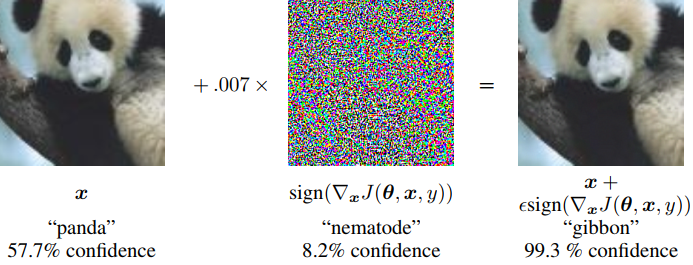
\includegraphics[width=3in]{fgsmEx.PNG}
\caption{An example of applying the FGSM algorithm \cite{Goodfellow2015ExplainingAH}}
\label{fgsmEx}
\end{figure}

\section{Methodology}
To make the generated adversarial examples more effective in fooling the network and more realistic from a human perspective, a network called Adv-GAN \cite{Xiao2018GeneratingAE} is used.

\subsection*{Problem Description}
Assume that $X \subseteq R^n$ is the feature space, $n$ is the number of features, $(x_i, y_i)$ is i-th example in the training dataset, consisting of feature vectors,
\begin{itemize}
\item $x_i \in X$: Generated based on an unknown distribution $x_i \sim P_{data}$;
\item $y_i \in Y$: The true and correct class label.
\end{itemize}

The goal of the learning system is to learn a classifier $f: X \rightarrow Y$ from the domain $X$ to the set of classification outputs $Y$. More specifically, given a sample $x$, the goal of the attacker is to generate an adversarial example $x_A$ such that $f(x_A) \neq y$ (in non-targeted attacks) or $f(x_A) = t$ (in targeted attacks), where $t$ is the target class, and $x_A$ is close to the original example $x$ in terms of the $L^2$ distance or other distance metrics.

\subsection*{Adv-GAN}
This network uses a feed-forward neural network to generate partial changes, and a discriminator network to guarantee the realism of generated samples. Compared to the FGSM, this approach allows for the immediate generation of adversarial examples for any input sample once the feed-forward network is trained. Therefore, without accessing the model itself (a semi-white-box attack) the adversarial sample can be generated. In addition, the Adv-GAN can be used for both white-box and black-box targeted and untargeted attacks.

The overall architecture of the Adv-GAN is illustrated in fig. \ref{advgan_arch}. The network consists of three neural networks:
\begin{enumerate}
\item The generator $G$
\item The discriminator $D$
\item The target neural network $f$
\end{enumerate}
The generator takes the original sample $x$ as input and produces a perturbation $G(x)$. Then $x + G(x)$ is fed to the discriminator $D$ to distinguish between the generated sample and the original sample. Here, the role of $D$ is to incentivize the generated samples to be indistinguishable from the original sample of that class. Finally, $x + G(x)$ is passed as input to $f$, which outputs its own loss $L_{adv}$ according to equation \ref{eq:f_loss} \cite{Xiao2018GeneratingAE}.

\begin{figure}[!t]
\centering
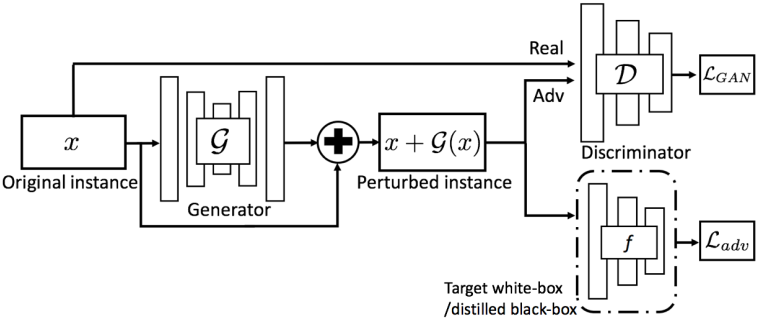
\includegraphics[width=3in]{advgan_arch.PNG}
\caption{The overall architecture of the Adv-GAN \cite{Xiao2018GeneratingAE}}
\label{advgan_arch}
\end{figure}

Equation \ref{eq:gan_loss} shows the adversarial loss:
\begin{equation} \label{eq:gan_loss}
L_{GAN} = \mathbb{E}_x log D(x) + \mathbb{E}x log (1- D(x + G(x)))
\end{equation}

Equation \ref{eq:f_loss} is used to calculate the loss for fooling the target model $f$ in a targeted attack:
\begin{equation} \label{eq:f_loss}
L^f{adv} = \mathbb{E}x l_f(x + G(x), t)
\end{equation}

It should be noted that the loss $L^f{adv}$ encourages the perturbed image to be misclassified into the target class $t$.
To limit the amound of perturbation, a \textit{Soft Hinge} loss on the $L_2$ norm is used in equation \ref{eq:soft_hinge_loss} where $c$ is a user-specified bound:
\begin{equation} \label{eq:soft_hinge_loss}
L_{hinge} = \mathbb{E}_x\:max(0, \|G(x)\|_2 - c)
\end{equation}

Therefore, the final objective (loss function) is given in equation \ref{eq:total_loss}:
\begin{equation} \label{eq:total_loss}
L = L^f_{adv} + \alpha L_{GAN} + \beta L_{hinge}
\end{equation}
where the parameters $\alpha$ and $\beta$ correspond to the importance of each objective.

Finally, $D$ and $G$ are obtained by solving a min-max game presented in equation \ref{eq:minmax_advgan}.
\begin{equation} \label{eq:minmax_advgan}
arg\:min_G\:max_D\:L
\end{equation}

\section{Results \& Discussion}
The codes were run on a GPU.1080Ti.xlarge with 31.3 GB of RAM and 6 virtual CPUs, running Ubuntu 18.04. The MNIST dataset, consisting of 60,000 28*28 pixel images for training the network and 10,000 28*28 pixel images for testing, were used. The hyper-parameters for training the target network are set to 60 epochs and a batch size of 128 (fig. \ref{target_model_arch}).

The generator network consists of three parts, including an encoder, bottleneck, and decoder. The encoder's architecture is shown in Fig. \ref{gen_arch_enc}, which is followed by the bottleneck part consisting of four identical Res-Net blocks whose architecture is shown in Fig. \ref{gen_arch_bottleneck}. The final part of the generator is the decoder, shown in Fig. \ref{gen_arch_dec}. 

The discriminator network architecture is shown in Fig. \ref{desc_arch}.

\subsection*{Target Network Before the Attack}
The performance of the target network before the attack is shown in Fig. \ref{before_targeted_model_accuracy} and Fig. \ref{before_targeted_model_loss}, where the accuracy and loss of the network are plotted against the training epochs. The network's accuracy and loss improve as the number of training epochs increases.
\begin{figure*}[!t]
\centering
\subfloat[]{
    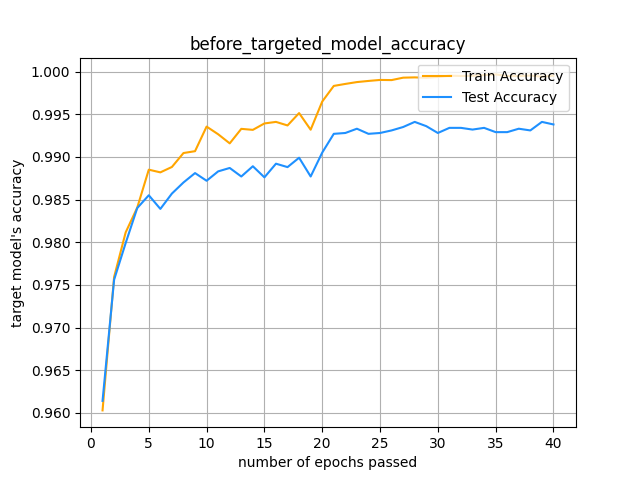
\includegraphics[width=3in]{before_targeted_model_accuracy}
    \label{before_targeted_model_accuracy}}
\subfloat[]{
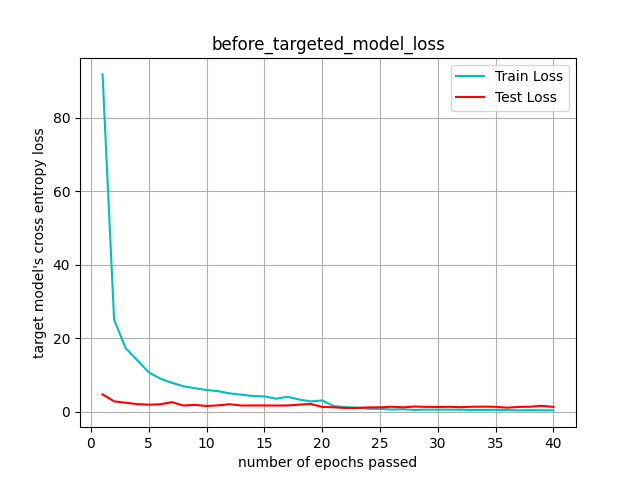
\includegraphics[width=3in]{before_targeted_model_loss}
    \label{before_targeted_model_loss}}
\caption{The accuracy and loss of the target network before the attack.}
\end{figure*}

Finally, after the completion of the target network training, its performance is evaluated on a test set containing 10,000 samples. The network classifies 70 samples incorrectly and accurately identifies 9930 samples (99.3\% accuracy) with a loss of 1.504620.

\subsection*{Adv-GAN}
Fig. \ref{discriminator_generator_GAN_model_performance} shows the loss for the generator and discriminator of the Adv-GAN network. As expected, the generator improves in generating more natural samples (loss closer to 1) and the discriminator performs better in distinguishing fake/generated samples from real/natural ones (loss closer to 0) as the network undergoes more training epochs.

In Fig. \ref{perturbation_GAN_model_performance}, the loss for the perturbation applied to the original image to generate adversarial samples is shown. As expected, the Adv-GAN network produces adversarial samples with less perturbation as it undergoes more training epochs, and thus, the generated samples become closer and more similar (loss closer to 0) to natural ones.

Fig. \ref{adversarial_GAN_model_performance} shows the adversarial loss, which is the main objective of the network to minimize. It can be observed that as the network undergoes more training epochs, adversarial samples can deceive the target network more and more and be classified into different categories from the original image. This loss actually shows the performance of the Adv-GAN network in fooling the target network, and the closer this loss is to 0, the weaker the target network becomes against attacks.

\begin{figure*}[!t]
\centering
\subfloat[]{
    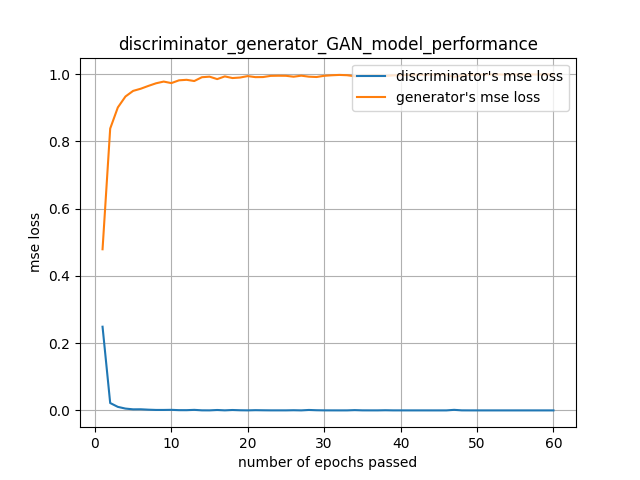
\includegraphics[width=2.2in]{discriminator_generator_GAN_model_performance}
    \label{discriminator_generator_GAN_model_performance}}
\subfloat[]{
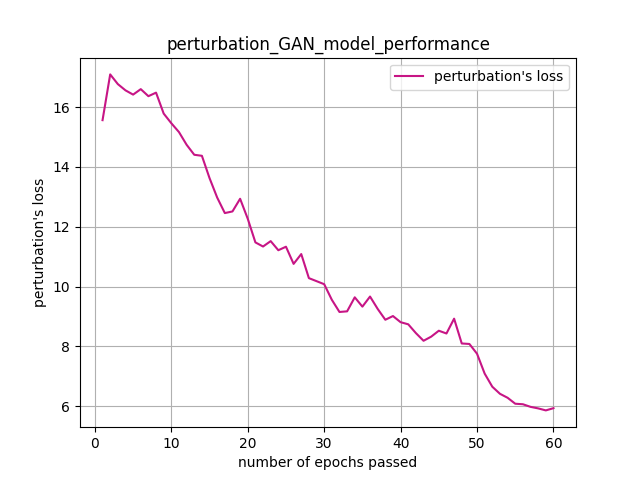
\includegraphics[width=2.2in]{perturbation_GAN_model_performance}
    \label{perturbation_GAN_model_performance}}
\subfloat[]{
    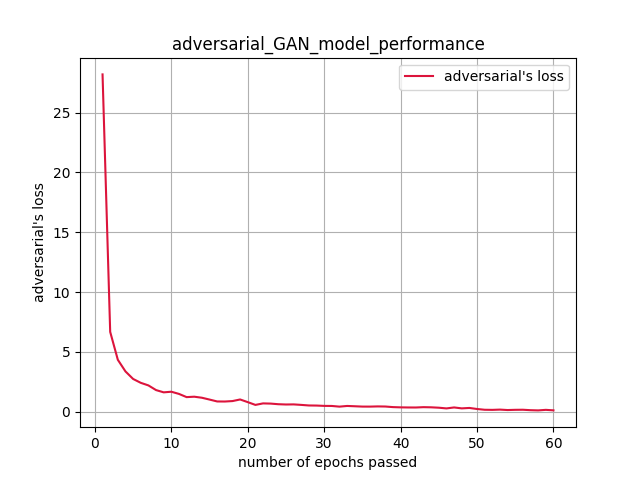
\includegraphics[width=2.2in]{adversarial_GAN_model_performance}
    \label{adversarial_GAN_model_performance}}
\caption{The performance of the Adv-GAN while training.}
\end{figure*}

\subsection*{Target Network After the Attack}
After training the Adv-GAN  and providing the adversarial examples generated by its generator  were fed to the target model, the results of the target network on the test dataset in Fig. \ref{testset_statistics}. The success rate of the attack is higher than 99.5\%, which means that the target network, which previously failed to correctly classify 70 cases in the testing dataset, now correctly classifies only about 43 cases.

\begin{figure}[!t]
\centering
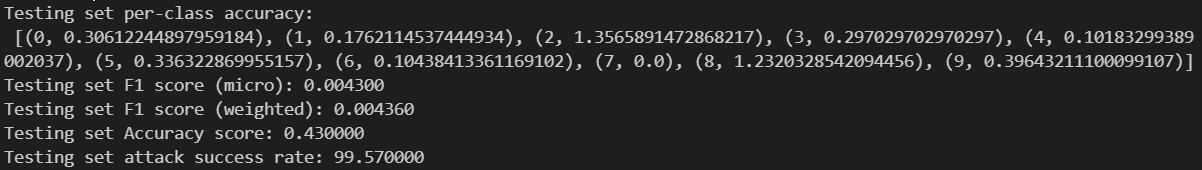
\includegraphics[width=3.3in]{testset_statistics.PNG}
\caption{Performance of the target network on the \textbf{testing} data after attack}
\label{testset_statistics}
\end{figure}

\subsection*{Adversarial Examples and Target Model}
After training the Adv-GAN network, the generator can be used separately which gets a random noise sample and produces an adversarial example.

In Fig. \ref{testset_imgs_matrix}, adversarial examples are shown for different original and predicted labels. In these figures, the rows indicate the original and true labels, and the columns indicate the predicted labels by the target model. Note that the empty spaces exist because the target model may never misclassify an image with the true label of 0 as the class 6, hence no adversarial example is generated for this case.

\begin{figure}[!t]
\centering
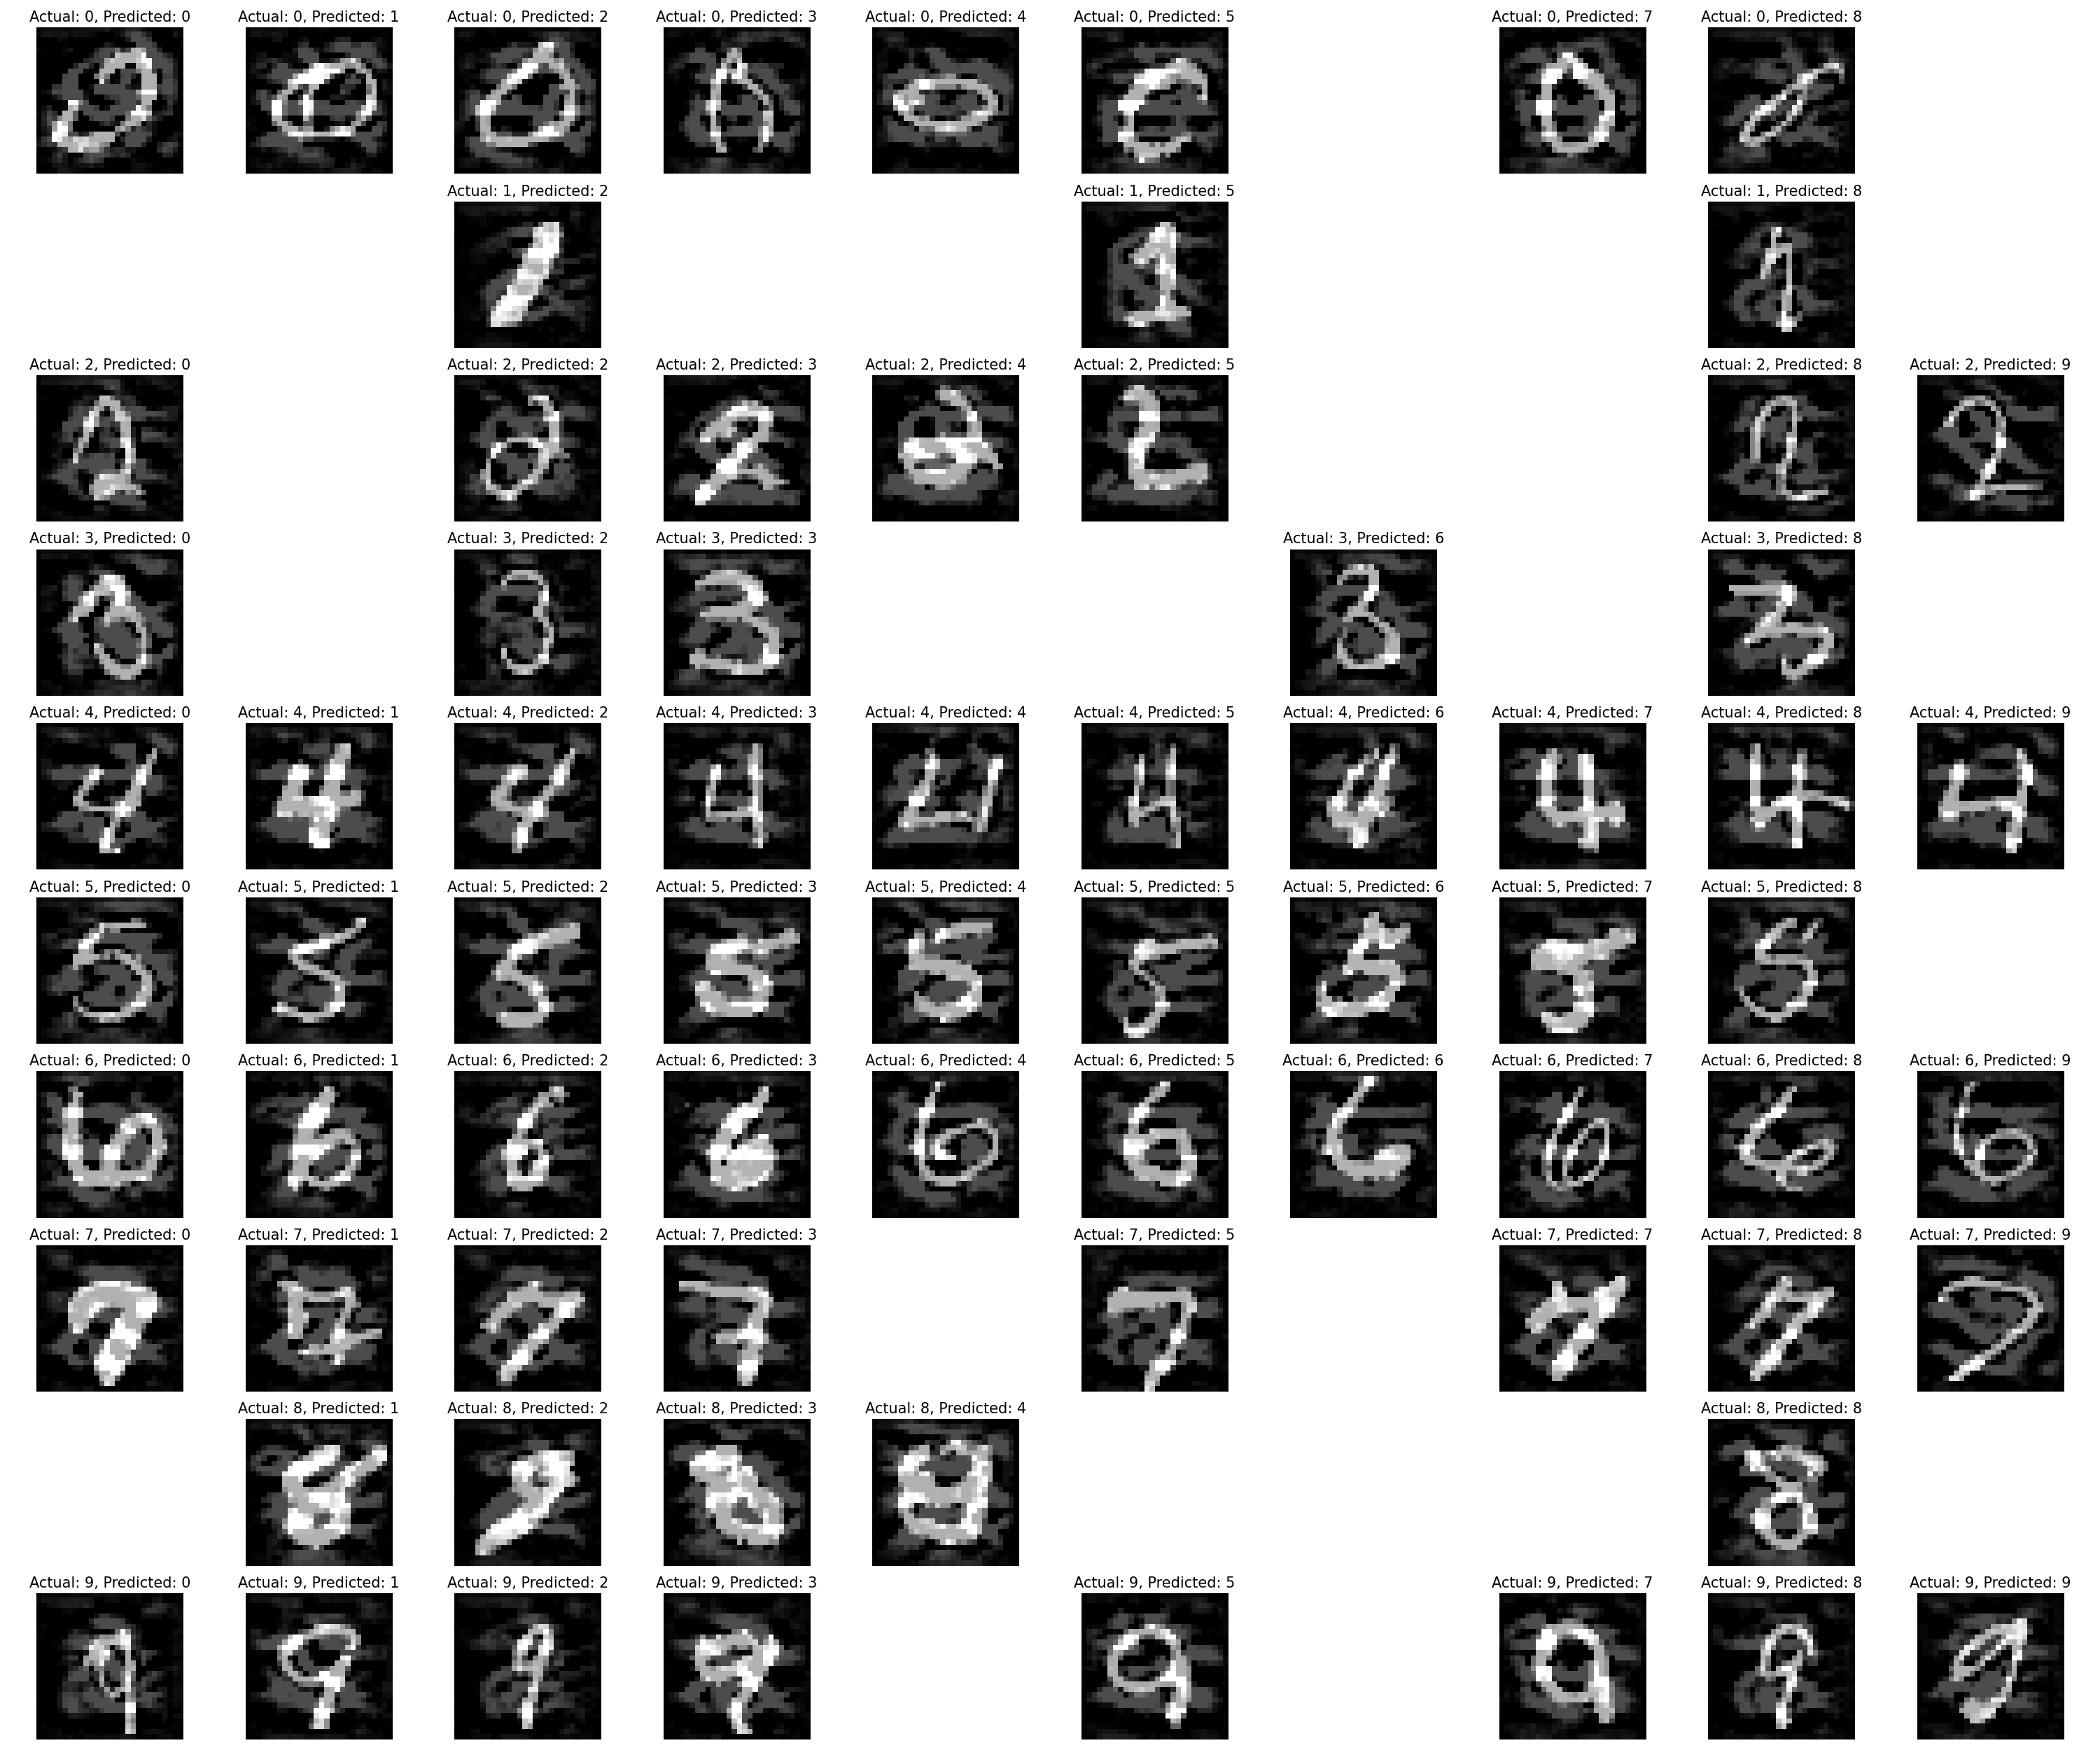
\includegraphics[width=3.3in]{testset_imgs_matrix.PNG}
\caption{Adversarial examples generated from test dataset images with original and predicted labels.}
\label{testset_imgs_matrix}
\end{figure}

Fig. \ref{testset_confusion_matrix} shows the confusion matrices obtained for the generated adversarial examples from test data, respectively. In these matrices, rows represent the true labels and columns represent the predicted labels by the target model. The diagonal elements of the matrix indicate the number of correct predictions for each label and class. As can be seen, most of the adversarial examples were classified into a wrong class. Additionally, it can be observed that, for example, most of the adversarial examples generated from class 1 training images were more similar to class 3 according to the target model.

\begin{figure}[!t]
\centering
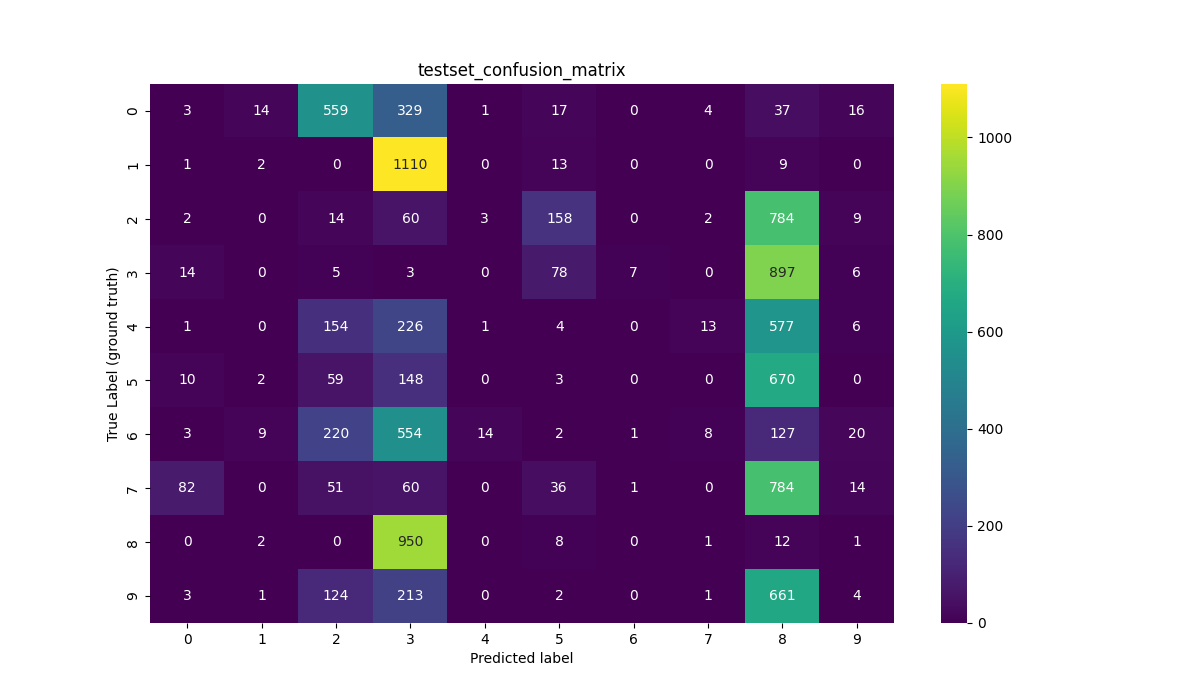
\includegraphics[width=3.3in]{testset_confusion_matrix.PNG}
\caption{Confusion matrix for adversarial examples generated from test data images.}
\label{testset_confusion_matrix}
\end{figure}

\section{Conclusion \& Future Work}
In this project, the Adv-GAN method was examined as a novel and powerful attack method against DNNs. The main idea of this network is inspired by GANs. Therefore, this method can be used in gray-box and black-box attacks with a high attack success rate because when the generator part of the Adv-GAN network is trained, it can independently produce optimal adversarial manipulations. The adversarial examples generated by this method have very high real quality, and therefore, this method is a strong candidate for evaluating DNNs against adversarial examples.
The trained network was able to reduce the performance of the target network from 99.3\% to a completely wrong performance of 0.43\%.
It is noteworthy that the existence of these adversarial examples shows that having high accuracy in explaining the dataset or even labeling it does not necessarily mean that the model has properly understood its task, and it is resistant to manipulated examples.

The vulnerability of neural networks to adversarial examples has led to very active research in the field of adversarial attacks and defense methods. In some research, techniques for defending neural networks against known attack methods are proposed, and in other areas, more powerful attack methods are being designed and presented. In some research, GANs have been used for both attacking and defending purposes. This extensive activity and effort will make DL methods much more resistant in the field of security and safety applications in the real world, and attackers will not be able to interfere and disrupt the network easily. Therefore, examining the performance of these attack methods on more complex and diverse datasets such as CIFAR-100 and ImageNet, as well as applying these attack methods on Recurrent networks and non-image textual datasets, is another step towards more reliable networks.

\bibliographystyle{IEEEtran}
\bibliography{IEEEabrv, MyReferences}

{\appendix[]
    \section*{Architecture of Neural Networks}
    
    \begin{figure}[!h]
    \centering
    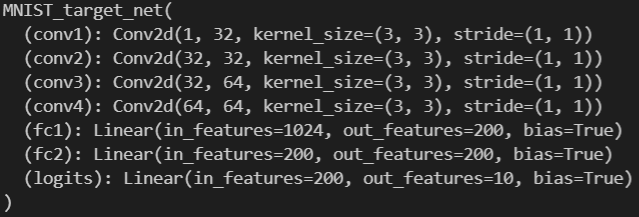
\includegraphics[width=3in]{target_model_arch.PNG}
    \caption{Architecture of target neural network}
    \label{target_model_arch}
    \end{figure}
    
    \begin{figure}[!h]
    \centering
    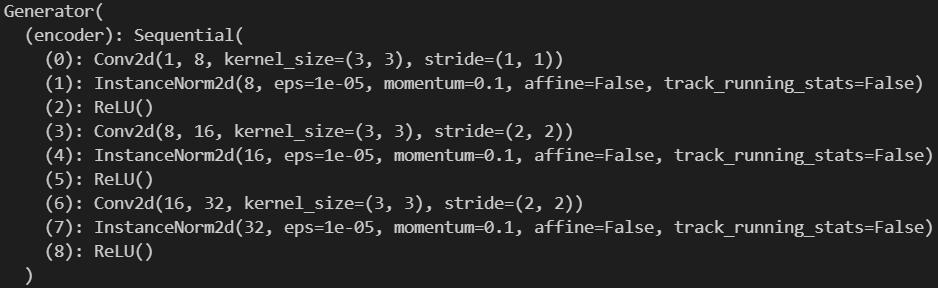
\includegraphics[width=3in]{gen_arch_enc.PNG}
    \caption{Architecture of the encoder in generator network}
    \label{gen_arch_enc}
    \end{figure}
    
    \begin{figure}[!h]
    \centering
    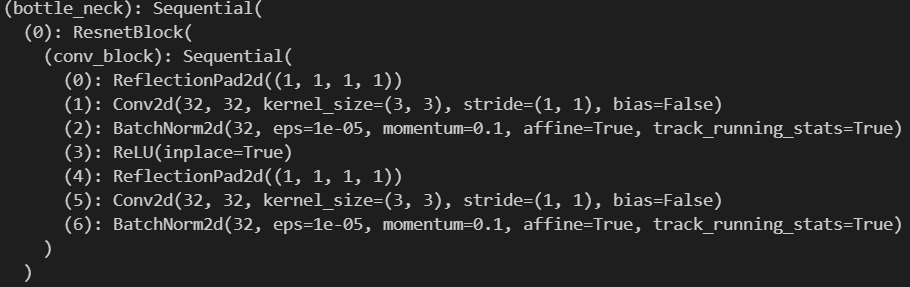
\includegraphics[width=3in]{gen_arch_bottleneck.PNG}
    \caption{Architecture of the bottleneck in generator network}
    \label{gen_arch_bottleneck}
    \end{figure}
    
    \begin{figure}[!h]
    \centering
    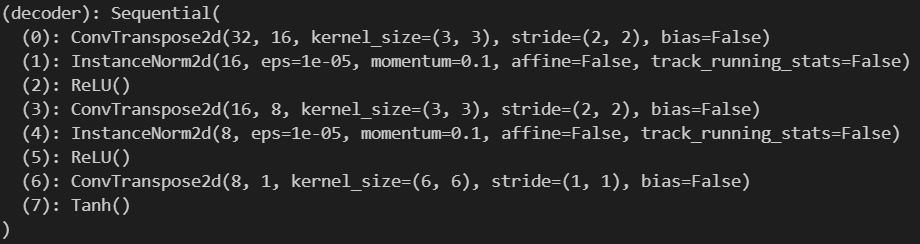
\includegraphics[width=3in]{gen_arch_dec.PNG}
    \caption{Architecture of the decoder in generator network}
    \label{gen_arch_dec}
    \end{figure}
    
    % \begin{figure*}[!t]
    % \centering
    % \subfloat[]{
    %     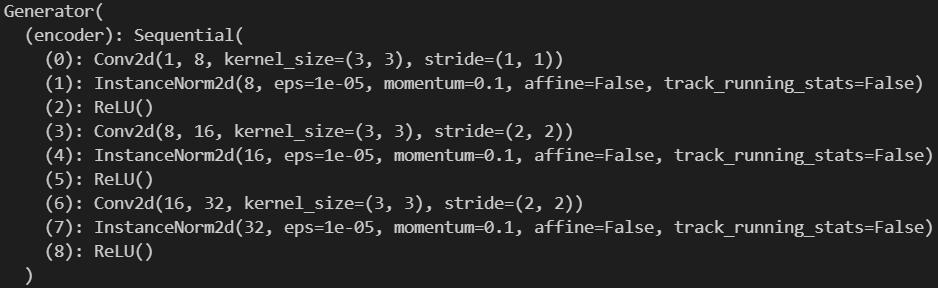
\includegraphics[width=2.2in]{gen_arch_enc}
    %     \label{gen_arch_enc}}
    % \subfloat[]{
    % 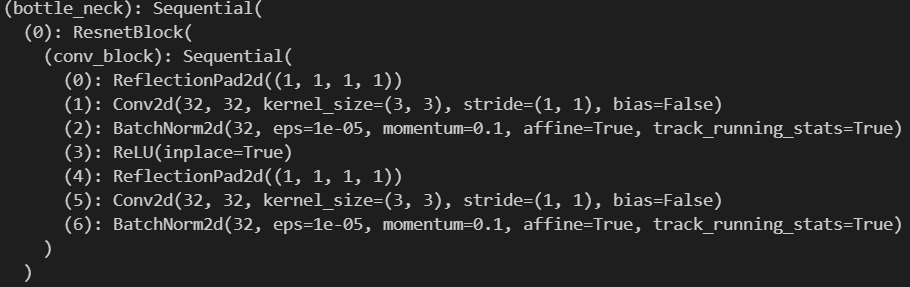
\includegraphics[width=2.2in]{gen_arch_bottleneck}
    %     \label{gen_arch_bottleneck}}
    % \subfloat[]{
    %     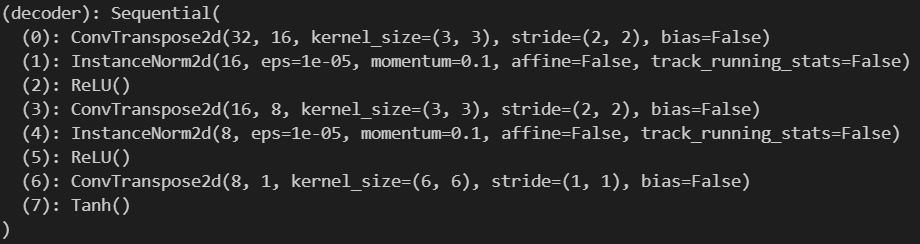
\includegraphics[width=2.2in]{gen_arch_dec}
    %     \label{gen_arch_dec}}
    % \caption{The architecture of the generator network.}
    % \end{figure*}
    
    \begin{figure}[!h]
    \centering
    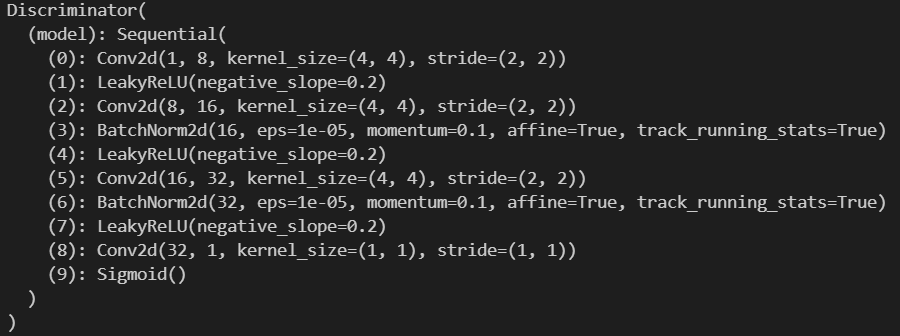
\includegraphics[width=3in]{desc_arch.PNG}
    \caption{Architecture of the discriminator network}
    \label{desc_arch}
    \end{figure}
    
}

\vfill

\end{document}
